\chapter{Gradient Descent và các biến thể}

% ==========================================
% SECTION 1: BÀI TOÁN
% ==========================================
\section{Bài toán tối ưu}
\begin{itemize}
    \item Xuất phát từ một điểm được coi là gần với nghiệm của bài toán, sau đó dùng phép toán lặp để tiến dần đến nghiệm cần tìm.
\end{itemize}

% ==========================================
% SECTION 2: GD CHO HÀM MỘT BIẾN
% ==========================================
\section{Gradient Descent cho hàm một biến}

\begin{figure}[H]
    \centering
    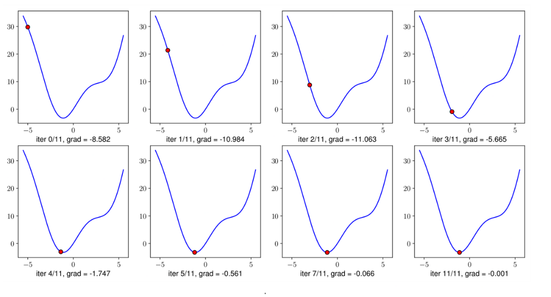
\includegraphics[width=0.8\linewidth]{61.png}
    %\fbox{\parbox[c][4cm][c]{0.8\linewidth}{\centering \textit{[Chèn ảnh: Minh họa Gradient Descent cho hàm 1 biến tại đây]}}}
    \caption{Cơ chế cập nhật điểm trong Gradient Descent một biến}
    \label{fig:gd_1d}
\end{figure}

\begin{itemize}
    \item \textbf{Công thức cập nhật:}
    \[
        x_{t+1} = x_t - \eta f'(x_t)
    \]
    trong đó $\eta$ là \textit{learning rate} (tốc độ học).
    \item Đi ngược hướng đạo hàm ($-f'(x_t)$) để tìm điểm có giá trị hàm mất mát nhỏ hơn.
    \item Mục tiêu là đưa $x$ về vị trí tối ưu $x^*$, nhưng ta không biết $x^*$ từ trước mà hoàn toàn phải tính toán dựa trên độ dốc hiện tại và tốc độ học.
    \item \textbf{Vai trò của đạo hàm $f'(x_t)$:} Chỉ rõ hướng và độ lớn của độ dốc, giúp tự động điều chỉnh bước nhảy:
    \begin{itemize}
        \item Khi còn xa đáy (điểm ở vị trí cao): độ dốc lớn $\rightarrow$ bước nhảy lớn để tiết kiệm thời gian.
        \item Càng gần về \textit{global minimum}: độ dốc nhỏ dần $\rightarrow$ bước nhảy nhỏ để tiến đến cực tiểu một cách thận trọng và chính xác hơn.
    \end{itemize}
    \item \textbf{Vai trò của Learning rate ($\eta$):} Thể hiện độ lớn bước nhảy / tốc độ di chuyển của điểm.
    \item Tốc độ hội tụ của Gradient Descent phụ thuộc vào cả \textbf{điểm xuất phát} và \textbf{learning rate}.
\end{itemize}

\begin{figure}[H]
    \centering
    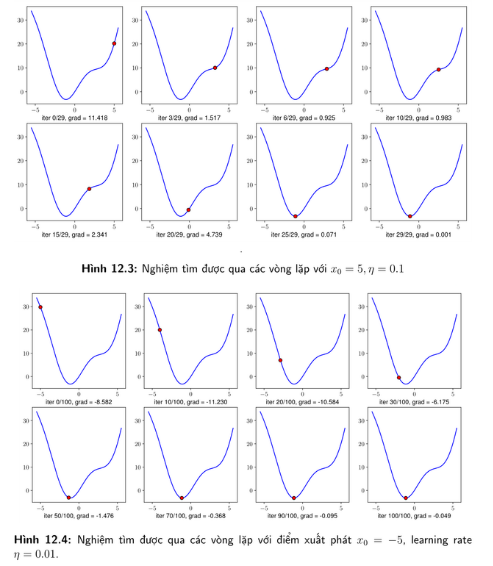
\includegraphics[width=0.8\linewidth]{62.png}
    %\fbox{\parbox[c][4cm][c]{0.8\linewidth}{\centering \textit{[Chèn ảnh: Minh họa Gradient Descent cho hàm 1 biến tại đây]}}}
    \caption{Cơ chế cập nhật điểm trong Gradient Descent một biến}
    \label{fig:gd_1d1}
\end{figure}

\begin{figure}[H]
    \centering
    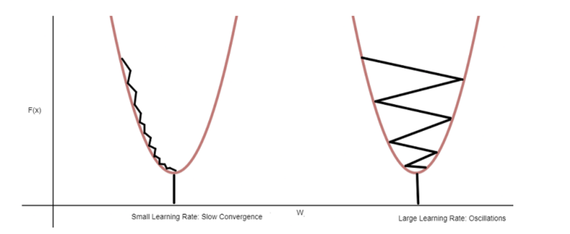
\includegraphics[width=0.8\linewidth]{64.png}
    %\fbox{\parbox[c][4cm][c]{0.8\linewidth}{\centering \textit{[Chèn ảnh: Minh họa Gradient Descent cho hàm 1 biến tại đây]}}}
    \caption{Cơ chế cập nhật điểm trong Gradient Descent một biến}
    \label{fig:gd_1d2}
\end{figure}
% ==========================================
% SECTION 3: GD CHO HÀM NHIỀU BIẾN
% ==========================================
\section{Gradient Descent cho hàm nhiều biến}

\begin{itemize}
    \item Là sự mở rộng trực tiếp từ trường hợp hàm một biến.
    \item Chuyển từ đạo hàm lên Gradient.
    \item Gradient: Tập hợp tất cả các đạo hàm riêng.
    \item \textbf{Biểu thức cập nhật:}
    \[
        \theta_{t+1} = \theta_t - \eta \nabla_\theta f(\theta_t)
    \]
\end{itemize}

% ==========================================
% SECTION 4: MOMENTUM
% ==========================================
\section{Gradient Descent với Momentum}

\begin{figure}[H]
    \centering
    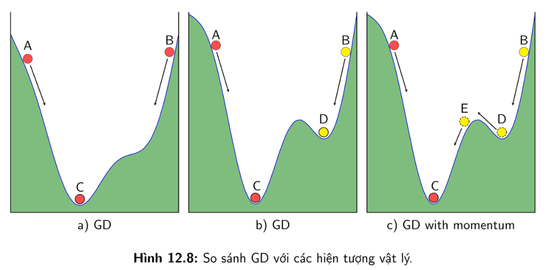
\includegraphics[width=0.8\linewidth]{65.png}
    %\fbox{\parbox[c][4cm][c]{0.8\linewidth}{\centering \textit{[Chèn ảnh: Minh họa Gradient Descent với Momentum tại đây]}}}
    \caption{Gradient Descent kết hợp Momentum vượt qua cực tiểu địa phương}
    \label{fig:gd_momentum}
\end{figure}

\begin{itemize}
    \item \textbf{Mục đích:} Giúp Gradient Descent thông thường thoát khỏi cực tiểu địa phương (\textit{local minimum}).
    \item \textbf{Ý tưởng:} Bổ sung thêm thành phần động lượng (xuất phát từ cơ học/động lực học) vào GD thông thường.
    \item \textbf{Công thức:}
    \[
        v_t = \gamma v_{t-1} + \eta \nabla_\theta J(\theta_t), \qquad \theta_{t+1} = \theta_t - v_t
    \]
    thực chất $v_t$ là một biến tích lũy (vận tốc).
    \item \textbf{Cơ chế triệt tiêu (giảm zigzag):} Nếu ở bước hiện tại điểm bị nhảy sang sườn dốc bên kia, hệ số $\gamma$ (thường chọn $\gamma = 0.9$) và $v_{t-1}$ sẽ giúp triệt tiêu thành phần dao động, làm $v_t$ nhỏ lại và hạn chế hiện tượng nhảy qua lại (zigzag).
    \item $v_t$ cộng dồn là một chuỗi hội tụ về $0$; khi đến đích vẫn có thể xảy ra một số lần đung đưa trước khi dừng hẳn.
    \item \textbf{Các trạng thái của $v_t$:}
    \begin{itemize}
        \item Lúc đầu ở trên đỉnh cao (độ dốc lớn), $v_t$ sẽ liên tục tăng tốc.
        \item $v_t$ bắt đầu giảm ngay khi lượng tăng thêm nhỏ hơn lượng thất thoát: $\eta \nabla_\theta J(\theta_t) < (1 - \gamma) v_{t-1}$.
        \item Đến một thời điểm khi $v_{t-1}$ quá lớn trong khi dốc thoải dần, $10\%$ thất thoát trở thành một con số lớn khiến lượng tăng thêm từ độ dốc không thể bù nổi vào.
    \end{itemize}
    \item \textbf{Nhược điểm:} Hiện tượng \textbf{Overshooting} (vượt quá đích do quán tính lớn).
\end{itemize}

% ==========================================
% SECTION 5: NESTEROV ACCELERATED GRADIENT (NAG)
% ==========================================
\section{Nesterov Accelerated Gradient (NAG)}

\begin{figure}[H]
    \centering
    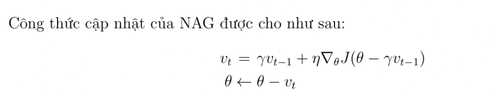
\includegraphics[width=0.8\linewidth]{67.png}
    %\fbox{\parbox[c][4cm][c]{0.8\linewidth}{\centering \textit{[Chèn ảnh: So sánh Momentum và Nesterov Accelerated Gradient tại đây]}}}
    \caption{Công thức cập nhật}
    \label{fig:gd_nag}
\end{figure}

\begin{itemize}
    \item \textbf{Mục đích chính:} Hạn chế hiện tượng \textit{overshooting} của Momentum.
    \item \textbf{Ý tưởng chính:} Dự đoán trước vị trí của nghiệm một bước.
    \item \textbf{Sự khác biệt giữa Momentum và NAG (nằm ở điểm lấy đạo hàm):}
    \begin{itemize}
        \item \textbf{Momentum:} Lấy đạo hàm tại vị trí hiện tại $\theta_t$ (kết hợp giữa momentum vector và gradient tại thời điểm hiện tại).
        \item \textbf{NAG:} Điểm lấy đạo hàm là vị trí dự đoán tiếp theo nếu đi theo momentum: $\theta_t - \gamma v_{t-1}$ (kết hợp giữa momentum vector và gradient tại vị trí dự đoán).
    \end{itemize}
    \item Nhờ đoán trước vị trí tiếp theo, NAG có cơ chế phanh/triệt tiêu mạnh hơn khi sắp vượt quá đích.
\end{itemize}

\begin{figure}[H]
    \centering
    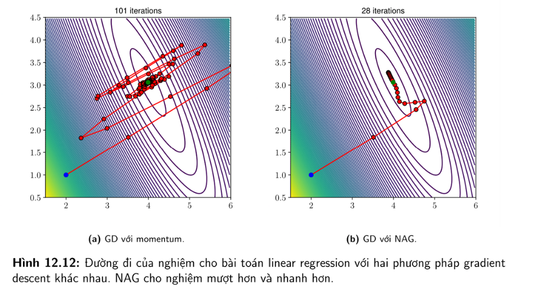
\includegraphics[width=0.8\linewidth]{68.png}
    %\fbox{\parbox[c][4cm][c]{0.8\linewidth}{\centering \textit{[Chèn ảnh: So sánh Momentum và Nesterov Accelerated Gradient tại đây]}}}
    \label{fig:gd_nag1}
\end{figure}

% ==========================================
% SECTION 6: BATCH, STOCHASTIC & MINI-BATCH GD
% ==========================================
\section{Các biến thể theo lượng dữ liệu cập nhật}

\subsection{Batch Gradient Descent}
\begin{itemize}
    \item Các thuật toán được đề cập ở các mục trước thuộc nhóm \textbf{Batch GD}.
    \item Khi cập nhật tham số $\theta$, thuật toán sử dụng \textbf{toàn bộ} các điểm dữ liệu $x_i$.
    \item \textbf{Hạn chế:} Với cơ sở dữ liệu lớn, việc tính toán trên toàn bộ dữ liệu cho mỗi bước cập nhật tốn rất nhiều thời gian.
\end{itemize}

\subsection{Stochastic Gradient Descent (SGD)}
\begin{itemize}
    \item Chấp nhận sai sót nhất định để đổi lấy hiệu quả tính toán cao.
    \item Tính đạo hàm tại \textbf{một điểm hoàn toàn ngẫu nhiên} rồi cập nhật tham số luôn, thay vì tính tại tất cả mọi điểm rồi lấy trung bình như GD nguyên thủy.
    \item Đạo hàm tại một điểm ngẫu nhiên được kỳ vọng là khá gần với đạo hàm trung bình của hàm mất mát trên toàn bộ dữ liệu.
    \item \textbf{Số lần cập nhật sau 1 epoch:} Là $N$ lần (so với GD nguyên thủy chỉ là $1$ lần). Tập dữ liệu được xáo trộn (shuffle) trước mỗi epoch.
    \item Để tránh hiện tượng dao động lặp lại quá nhiều quanh cực tiểu, SGD thường kết hợp với kỹ thuật \textbf{Learning Rate Decay} (giảm dần tốc độ học theo thời gian).
\end{itemize}

\subsection{Mini-batch Gradient Descent}
\begin{itemize}
    \item Kết hợp và tối ưu giữa Batch GD nguyên thủy (quá chậm) và SGD (quá nhiễu).
    \item Chia tập dữ liệu lớn ($N$ phần tử) thành nhiều tập nhỏ (mỗi tập có $k$ phần tử), tính toán và cập nhật tham số trên từng tập nhỏ đó $\rightarrow$ một epoch có $N/k$ lần cập nhật.
    \item \textbf{Ưu điểm:} Giảm thiểu sai sót/nhiễu của SGD và tăng tốc độ, số lần cập nhật so với Batch GD.
\end{itemize}

\begin{figure}[H]
    \centering
    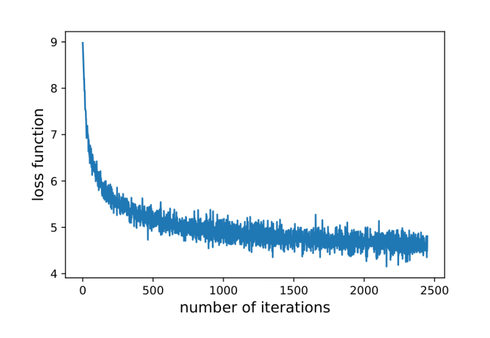
\includegraphics[width=0.8\linewidth]{69.png}
    %\fbox{\parbox[c][4cm][c]{0.8\linewidth}{\centering \textit{[Chèn ảnh: So sánh Momentum và Nesterov Accelerated Gradient tại đây]}}}
    \caption{Mini-batch visualization}
    \label{fig:mnb_visualization}
\end{figure}


\begin{figure}[H]
    \centering
    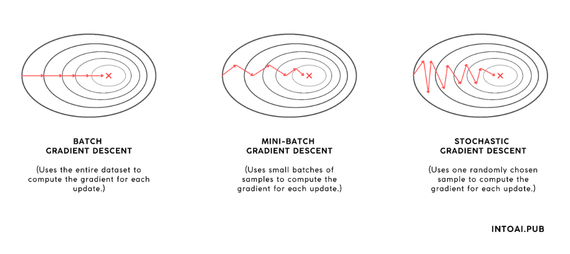
\includegraphics[width=0.8\linewidth]{610.png}
    %\fbox{\parbox[c][4cm][c]{0.8\linewidth}{\centering \textit{[Chèn ảnh: So sánh Momentum và Nesterov Accelerated Gradient tại đây]}}}
    \caption{Tương quan giữa các phương pháp}
    \label{fig:tuongquan}
\end{figure}

% ==========================================
% SECTION 7: THỜI ĐIỂM DỪNG THUẬT TOÁN
% ==========================================
\section{Thời điểm dừng thuật toán (Stopping Criteria)}

\begin{itemize}
    \item \textbf{Giới hạn số vòng lặp:} Đặt trước số epoch/iteration tối đa. Hạn chế là dễ dừng ở thời điểm chưa tối ưu.
    \item \textbf{So sánh gradient (độ dốc):} So sánh giá trị gradient của nghiệm giữa hai lần cập nhật liên tiếp, khi đủ nhỏ thì dừng. Hạn chế là đôi khi việc tính đạo hàm phức tạp.
    \item \textbf{So sánh giá trị hàm mất mát (độ cao):} So sánh giá trị hàm mất mát tại hai thời điểm cập nhật liên tiếp, khi độ chênh lệch đủ nhỏ thì dừng.
    \item \textbf{Early Stopping (Kiểm tra định kỳ):} Cho thuật toán chạy với số vòng lặp rất lớn; trong quá trình chạy, thường xuyên kiểm tra chất lượng mô hình trên tập huấn luyện và/hoặc tập validation để dừng đúng lúc.
\end{itemize}